%; whizzy paragraph -pdf xpdf -latex ./whizzypdfptex.sh
%; whizzy-paragraph "^\\\\begin{frame}\\|\\\\emtext"
% latex beamer presentation.
% platex, latex-beamer でコンパイルすることを想定。 

%     Tokyo Debian Meeting resources
%     Copyright (C) 2012 Junichi Uekawa

%     This program is free software; you can redistribute it and/or modify
%     it under the terms of the GNU General Public License as published by
%     the Free Software Foundation; either version 2 of the License, or
%     (at your option) any later version.

%     This program is distributed in the hope that it will be useful,
%     but WITHOUT ANY WARRANTY; without even the implied warreanty of
%     MERCHANTABILITY or FITNESS FOR A PARTICULAR PURPOSE.  See the
%     GNU General Public License for more details.

%     You should have received a copy of the GNU General Public License
%     along with this program; if not, write to the Free Software
%     Foundation, Inc., 51 Franklin St, Fifth Floor, Boston, MA  02110-1301 USA

\documentclass[cjk,dvipdfmx,12pt]{beamer}
\usetheme{Tokyo}
\usepackage{monthlypresentation}

%  preview (shell-command (concat "evince " (replace-regexp-in-string "tex$" "pdf"(buffer-file-name)) "&")) 
%  presentation (shell-command (concat "xpdf -fullscreen " (replace-regexp-in-string "tex$" "pdf"(buffer-file-name)) "&"))
%  presentation (shell-command (concat "evince " (replace-regexp-in-string "tex$" "pdf"(buffer-file-name)) "&"))

%http://www.naney.org/diki/dk/hyperref.html
%日本語EUC系環境の時
\AtBeginDvi{\special{pdf:tounicode EUC-UCS2}}
%シフトJIS系環境の時
%\AtBeginDvi{\special{pdf:tounicode 90ms-RKSJ-UCS2}}

\newenvironment{commandlinesmall}%
{\VerbatimEnvironment
  \begin{Sbox}\begin{minipage}{1.0\hsize}\begin{fontsize}{8}{8} \begin{BVerbatim}}%
{\end{BVerbatim}\end{fontsize}\end{minipage}\end{Sbox}
  \setlength{\fboxsep}{8pt}
% start on a new paragraph

\vspace{6pt}% skip before
\fcolorbox{dancerdarkblue}{dancerlightblue}{\TheSbox}

\vspace{6pt}% skip after
}
%end of commandlinesmall

\title{東京エリアDebian勉強会}
\subtitle{第129回 2015年8月度}
\author{野島貴英}
\date{2015年8月22日}
\logo{
\includegraphics[width=8cm]{image200607/openlogo-light.eps}}

\begin{document}

\begin{frame}
\titlepage{}
\end{frame}

\begin{frame}{設営準備にご協力ください。}
会場設営よろしくおねがいします。
\end{frame}

\begin{frame}{Agenda}
 \begin{minipage}[t]{0.45\hsize}
  \begin{itemize}
   \item 注意事項
	 \begin{itemize}
	  \item 写真はセミナールーム内のみ可です。
          \item 出入りは自由でないので、もし外出したい方は、野島まで一声くださいませ。
	 \end{itemize}
   \item 事前課題発表
  \end{itemize}
 \end{minipage} 
 \begin{minipage}[t]{0.45\hsize}
  \begin{itemize}
   \item 最近あったDebian関連のイベント報告
	 \begin{itemize}
	 \item 第128回 東京エリアDebian勉強会
	 \end{itemize}
   \item APT1.1 超☆牛さんパワー炸裂!
   \item 今後のイベント
   \item 今日の宴会場所
  \end{itemize}
 \end{minipage}
\end{frame}

\section{事前課題}
\emtext{事前課題}
{\footnotesize
\begin{prework}{ 野島 }
  \begin{enumerate}
  \item Q.hack timeに何をしますか?\\
    A. 今度こそ!Nook HD+をDebianに。
  \item (オプション)Q.何について聞きたい/参加者と話をしたいですか?\\
    A. 俺とDebian
  \end{enumerate}
\end{prework}

\begin{prework}{ zinrai }
  \begin{enumerate}
  \item Q.hack timeに何をしますか?\\
    A. mincsのITP。https://github.com/mhiramat/mincs
  \end{enumerate}
\end{prework}

\begin{prework}{ wskoka }
  \begin{enumerate}
  \item Q.hack timeに何をしますか?\\
    A. tilegxへの移植
  \item (オプション)Q.どこで今回の勉強会の開催を知りましたか?\\
    A. その他
  \end{enumerate}
\end{prework}

\begin{prework}{ issei }
  \begin{enumerate}
  \item Q.hack timeに何をしますか?\\
    A. dgitの使い方をマスターする。
  \end{enumerate}
\end{prework}

\begin{prework}{ khibino }
  \begin{enumerate}
  \item Q.hack timeに何をしますか?\\
    A. Debian haskell チームへの参加について調べる
  \item (オプション)Q.どこで今回の勉強会の開催を知りましたか?\\
    A. 友達や知り合いから直接
  \end{enumerate}
\end{prework}

\begin{prework}{ Roger Shimizu }
  \begin{enumerate}
  \item Q.hack timeに何をしますか?\\
    A. Debian BTSの確認など
  \item (オプション)Q.どこで今回の勉強会の開催を知りましたか?\\
    A. その他
  \end{enumerate}
\end{prework}


\begin{prework}{yy\_y\_ja\_jp}
  \begin{enumerate}
  \item Q.hack timeに何をしますか?\\
    A. DDTSS\\
    http://ddtp.debian.net/ddtss/index.cgi/ja
  \item (オプション)Q.何について聞きたい/参加者と話をしたいですか?\\
    A. DDTSS
  \item (オプション)Q.どこで今回の勉強会の開催を知りましたか?\\
    A. その他
  \end{enumerate}
\end{prework}



}

\section{イベント報告}
\emtext{イベント報告}

\begin{frame}{第128回東京エリアDebian勉強会}

\begin{itemize}
\item 場所はスクウェア・エニックスさんのセミナルームをお借りしての開催でした。
\item 参加者は6名でした。
\item セミナ内容は野島さんによる「DebianでHTTP/2を試す」でした。
\item 残りの時間でhack timeを行い、成果発表をしました。
\item 宴会の代わりに、「中国料理 東順永 本店」で夕食会をやりました。
\end{itemize} 
  
\end{frame}

\begin{frame}{第128回東京エリアDebian勉強会(つづき)}

  セミナは野島さんより、DebianでHTTP/2を試す事について発表がありました。内容としては、HTTP/2の規格概要、デモ、Debianで最も簡単にHTTP/2対応サーバを動かしてみる等となりました。

  今年RFC化される、あるいは、某有名携帯端末の会社のイベントでHTTP/2を使って欲しいアピールがあったなど、HTTP/2が少しづつ推される(あるいはいつの間にか使っている?)場面も、今後増えてくるかと思います。Debianがあればサーバ稼働も含めてすぐに試せますので、皆様も是非!

\end{frame}

\begin{frame}{第128回東京エリアDebian勉強会(つづき)}

  また、参加者の中で、hacktime中に書いたLinux Kernel向けパッチが取り込まれた、Bug Reportした内容がLWN/Gigazineに取り上げられた等、いろいろな形で成果を出された旨の報告がありました。こういった方々がいらっしゃるのは正直凄い事だと思います。

\end{frame}

\begin{frame}{第128回東京エリアDebian勉強会(つづき)}
  
  Debianは多様性をモットーとしているコミュニティでもあります。参加したいと思った方々には、IT技術面・非IT技術面、どちらも十分に活躍して成果をうたえる余地にあふれ、万年人手不足のコミュニティです。参加された方々におきましては、様々な形でいつでも頭角を表していただけるチャンスにあふれてますので、皆様も是非!

\end{frame}

\section{APT1.1 超☆牛さんパワー炸裂!}
\emtext{APT1.1 超☆牛さんパワー炸裂!}

\begin{frame}{はじめに}

  debian-devel-announceに、''Moo! 9th preview of APT 1.1 released: Go and test new supercow powers''というタイトルで、APT 1.1のアナウンスが流れました。

  今回は、Debianの重要なツールの1つであるAPTについて、1.1に搭載された特徴をネタにディスカッションしてみようと思います。
  
\end{frame}

\begin{frame}{Debconf15でも}

  今回のdebian-devel-announceでも触れられていますが、2015/8/15-8/22にて、ドイツのHeidelbergで開催中のDebConf15にても、APT1.1のセッションが開かれました。

  ビデオ:''This\_APT\_has\_Super\_Cow\_Powers''\\
  \url{http://meetings-archive.debian.net/pub/debian-meetings/2015/debconf15/This_APT_has_Super_Cow_Powers.webm}
  
\end{frame}

\begin{frame}[containsverbatim]{早速評価してみる!}

\begin{commandlinesmall}
$ sudo vi /etc/apt/source.lists
deb http://ftp.jp.debian.org/debian/ experimental main contrib non-free
deb-src http://ftp.jp.debian.org/debian/ experimental main contrib non-free
$ sudo apt-get update
$ sudo apt-get -t experimental install apt
$ apt
apt 1.1~exp9 (amd64)
Usage: apt [options] command
...中略...
 full-upgrade - upgrade the system by removing/installing/upgrading packages
 edit-sources - edit the source information file
\end{commandlinesmall}
\begin{center}
{\LARGE 動いた!}
\end{center}
\end{frame}

\begin{frame}{APT 1.1の特徴は?}

 jessie搭載のAPT 1.0.9.8に比べての違いを述べていきます。

\end{frame}

\begin{frame}{APT 1.1の特徴は?(概要から)}

 先に紹介したDebConf15のビデオを見ると以下の点が変更点概要となります。

\begin{itemize}
\item リポジトリの情報のセキュリティ検証がとても強化された。
\item deb822形式でリポジトリを指定するやり方にて機能強化。(/etc/apt/*.sourcesファイル)
\item httpredir.debian.orgを受けて、処理の途中経過の表示を変更。
\item Pinningがちゃんと(笑)動くようになった。
\item 依存関係をする場合、ローカルにおいた.debファイルを直接指定してもインストールでき、ソースビルドの依存関係を指定する方法が柔軟になった。
\end{itemize}

\end{frame}  

\begin{frame}{APT 1.1の特徴は?(manから)}

  manからみた1.0.9.8との違いのうち、
  \begin{itemize}
  \item aptコマンド
  \item apt-getコマンド
  \end{itemize}
  についてここでは述べてみます。
\end{frame}

\begin{frame}{APT 1.1の特徴は?(manから)}

  まずはman aptで見た1.0.9.8との違いから...

 \begin{itemize}
 \item autoremove \\
   依存関係を満たすためだけにインストールされたパッケージがあるとします。ここで、現在はその依存関係からも外されており、もはや全く使われていないパッケージがあります。このコマンドをつけてaptコマンドを起動すると、こういった使われていないパッケージを削除することが出来ます。
 \end{itemize}
\end{frame}

\begin{frame}{autoremove仕組み}

  もちろん、パッケージの中には、利用者が自分で明示して入れたパッケージもあり、必ずしも他のパッケージで依存していなからといってautoremoveで消されたら困ってしまいます。

\end{frame}

\begin{frame}{autoremove仕組み(つづき1)}
  自動で消してもよいか?についての判断基準:

\begin{description}
 \item [Step 1.] /var/lib/apt/extended\_statesファイルの記録に、過去、依存関係を満たすためにパッケージを導入したかどうかの記録である''Auto-Installed: 1''と記されているパッケージを候補とする。
 \item [Step 2.] すでにインストール済パッケージのどれからも依存関係に無いかどうか?
  \end{description}

\end{frame}

\begin{frame}{autoremove仕組み(つづき2)}

\begin{description}
 \item [Step 3.] さらに、
\begin{itemize}
\item Recommendsとして提案されているパッケージはインストールして欲しいと明示した場合、
\item Suggestとして提案されているパッケージはインストールして欲しいと明示した場合、
\end{itemize}
のいずれにも該当していないか?
  \end{description}

 の場合、自動削除候補のパッケージとなります。

  
\end{frame}


\begin{frame}{APT 1.1の特徴は?(manから)}

  次にman apt-getで見た1.0.9.8との違いから...
 \begin{itemize}
\item indextargets \\
   apt-get updateで更新されるファイルと状態をdeb822形式で表示します。
 \item --allow-downgrades \\
   特定パッケージをダウングレードすることにより依存関係が満たせるときに、ユーザに尋ねず実行してまうというオプションです。
 \end{itemize}
\end{frame}

\begin{frame}{APT 1.1の特徴は?(manから)}

\begin{itemize}
 \item --allow-remove-essential \\
   何らかの理由によりDebianシステムの必須パッケージ(essentialパッケージとして分類されている)ものを消せば依存関係が満たせるときに、消してよいか?を尋ねず消してしまうオプションです。
 \item --allow-change-held-packages \\
  何らかの理由によりHold扱いにしたパッケージを削除すれば依存関係が満たせるときに、消してよいか?を尋ねず消してしまうオプションです。
 \item --no-allow-insecure-repositories \\
   リポジトリにあるReleaseファイル(InReleaseファイル)のGPGによる署名が確認出来ない等、セキュリティ上問題があるとみなされたリポジトリが含まれた場合、apt-get update操作を失敗させます。
\end{itemize}

\end{frame}

\begin{frame}[containsverbatim]{牛さんパワー}

  apt/apt-getコマンドには''moo''というmanには無いオプションがあります。
以下にaptの場合の起動方法を載せます。
\begin{commandlinesmall}  
$ apt moo 
$ apt moo moo [--color]
$ apt moo moo moo  
$ faketime '1997-04-01' apt moo
\end{commandlinesmall}    
  
\end{frame}

\begin{frame}{牛さんパワー(つづき)}

\begin{figure}[H]
\begin{center}
 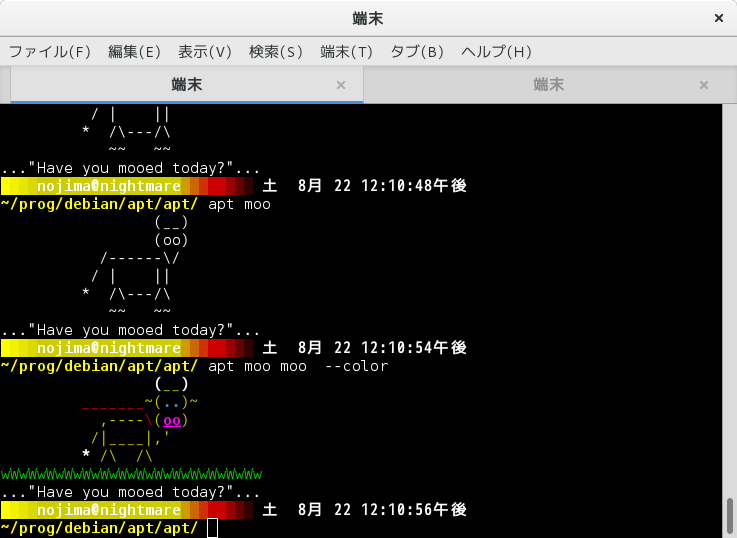
\includegraphics[width=1.0\hsize]{image201508/apt-moo.png}
\end{center}
\caption{apt mooコマンド結果例}
\end{figure}

\end{frame}

\begin{frame}[containsverbatim]{リポジトリ堅牢化}

  今回、APT 1.1はリポジトリのセキュリティの正当性評価が強化されているのですが、こちらの元となるファイルにReleaseファイル(InReleaseファイル)があります。

\begin{commandlinesmall}
$ curl http://cloudfront.debian.net/debian/dists/unstable/InRelease
-----BEGIN PGP SIGNED MESSAGE-----
Hash: SHA256

Origin: Debian
Label: Debian
...中略...
MD5Sum:
 e9f9b477f2430a7d0e2dd686da1af507 30975818 Contents-amd64.gz
 d158f809191a841bedf9ff50e34e0ebe 30421142 Contents-armel.gz
...中略...
-----BEGIN PGP SIGNATURE-----
Version: GnuPG v1

iQIcBAEBCAAGBQJV1+IMAAoJEItIrWJGklVTgloP/0+XAch/TMtTSfH+N1QFl+q2
Woas1LpWhHDO12U6vuPq5wghCPYE5ctNuDxFtTy9j01lsf6kWXPDh1QupNENDNHr
lfZ7Qa9gFr8W3tH1tnPwsSqcQmu9bMkR0sRDVSfcFlDioVhN/h+jWW7j7J7nrZrE
...中略...
\end{commandlinesmall}
  
\end{frame}

\begin{frame}{リポジトリ堅牢化(つづき)}

  みるとわかるとおり、

\begin{itemize}
\item リポジトリに含まれる様々なファイルは全てmd5sum付きでInReleaseファイルに記録
\item さらにInReleaseファイルも電子署名による正当性確認が出来るようになっている
\end{itemize}

 となります。

 今回APT1.1では、基本的にInReleaseファイルの無い、あるいは、他に必要なファイルが欠落しているなど、セキュリティ観点からの正当性確認が出来ないリポジトリは取り扱いを完全にやめる設計にした模様。
  
\end{frame}
  
\begin{frame}{httpredir.debian.org対応}

  2015/5月頃、Debianユーザに最も近いmirrorサーバーをHTTP Redirectでaptに教えてくれるサービスが稼働しました。つまり、ユーザは/etc/apt/sources.listに、httpredir.debian.orgを指定すれば、ユーザに最も近いmirrorサーバーへリダイレクトされます。

  ここで、リダイレクトされた結果どこのサーバから取得するのか?がわかると便利な事が多いです。このため、APT1.1のapt/apt-getはリダイレクトされた先の情報を表示するように変更されました。
  
\end{frame}

\begin{frame}[containsverbatim]{httpredir.debian.orgの様子}

\begin{commandlinesmall}
$curl -v http://httpredir.debian.org/debian/dists/sid/InRelease
> GET /debian/dists/sid/InRelease HTTP/1.1
> Host: httpredir.debian.org
> User-Agent: curl/7.44.0
> Accept: */*
> 
< HTTP/1.1 302 Found
< Date: Sat, 22 Aug 2015 03:54:12 GMT
< Location: http://cloudfront.debian.net/debian/dists/sid/InRelease
< Content-Type: text/plain
...省略...
\end{commandlinesmall}    

 cloudfront.debian.netにリダイレクトで飛ばされるのが確認できると思います。

\end{frame}

\begin{frame}{ここで横道:え?cloudfront?}

 前ページのリダイレクト先にて、\\
\url{http://cloudfront.debian.net/}
とリポジトリが提案されています。これは、2年前にdebian-cloudチームでアナウンスがあった、
\url{https://lists.debian.org/debian-cloud/2013/05/msg00066.html}
AWSのcloudfrontというCDNの仕組みを使ってデータ配布を行う試みのリポジトリです。

\end{frame}

\begin{frame}{ここで横道:え?cloudfront?(つづき)}

 もともと、CDNはユーザに最も効率的なサーバを提示してデータを配る仕組みであり、
AWSのcloudfrontは相当な規模とサービスエリアを持つCDNサービスですので、
そもそもこちらがあるなら、AWSのサービスがカバーしている国では、httpredir.debian.orgを
使わなくてすみそうな気もします。
    
\end{frame}

\begin{frame}[containsverbatim]{deb822って??}

  APT1.1が手元にあれば、簡単に表示させる事が出来ます。

\begin{commandlinesmall}  
$ apt-get indextargets
MetaKey: main/source/Sources
ShortDesc: Sources
Description: http://ftp.jp.debian.org/debian sid/main Sources
URI: http://ftp.jp.debian.org/debian/dists/sid/main/source/Sources
Filename: /var/lib/apt/lists/ftp.jp.debian.org_debian_dists_sid_main_source_Sources
Optional: no
Codename: sid
...中略...
\end{commandlinesmall}  
  
\end{frame}

\begin{frame}{deb822って??(つづき)}

  フォーマットを見るとわかるのですが、RFC822ヘッダの形式によく似ています。ここから、deb822と名前を取ったようです。

  特徴として、RFC822と同様ですので、ヘッダを増やせば、簡単に機能拡張できるという点が上げられます。

  また、動作未確認ですが、DebConf15のビデオによれば、
\begin{quote}
  /etc/apt/source.list.d/xxxx.sources
\end{quote}
(末尾が、.sourcesである事が必要)という名前でdeb822形式で置いておくと、
こちらをsources.listに指定したのと同様の動作をapt/apt-getは行うようです。
\end{frame}


\begin{frame}{おわりに}

  まだまだ、APT1.1について、今回ここでは書ききれない程の変更が加えられているようです。gitで落として差分を確認しましたが、実に2万行を超える変更が行われていました。
  
  正式リリースになるとドキュメントも揃ってくることが期待できそうです。将来、ドキュメントが充実することを期待しています。
  
\end{frame}

\section{今後のイベント}
\emtext{今後のイベント}
\begin{frame}{今後のイベント}
\begin{itemize}
 \item 関西エリアDebian勉強会
 \item 9/5(土) 10:00- OSC 2015 Niigataでセミナ&ブース\\
\url{http://www.ospn.jp/osc2015-niigata/}
 \item 9/12(土) 10:00- 東京エリアDebian勉強会 パッケージング道場(←仮題。東京)
\end{itemize}
\end{frame}

\begin{frame}{宣伝:パッケージング道場}

 \begin{itemize}
  \item 毎年恒例のDebian公式開発者(岩松)直伝によるパッケージング道場が開催されます!
  \item Debianの動くノートPCさえあれば誰でも参加可能です。
  \item Debianの公式パッケージの出し方を一気に習得できるチャンスです!そこの貴方も是非(笑)
 \end{itemize}

\end{frame}
  
\section{今日の宴会場所}
\emtext{今日の宴会場所}
\begin{frame}{今日の宴会場所}
未定
\end{frame}

\end{document}

;;; Local Variables: ***
;;; outline-regexp: "\\([ 	]*\\\\\\(documentstyle\\|documentclass\\|emtext\\|section\\|begin{frame}\\)\\*?[ 	]*[[{]\\|[]+\\)" ***
;;; End: ***
